

% ==============================================================================
%\chapter*{\vspace{-1.0cm}Introduction}   \addcontentsline{toc}{chapter}{Introduction} \label{intro}
\chapter{Phonon Decoherence}   \label{wigner}
% ==============================================================================


\section{Introduction}
The Phonon Decoherence (PD) tool comprises methods, approaches and algorithms for particle simulation of quantum decoherence in the phase space. The theoretical foundation for the implemented algorithms is the Wigner description from the field of quantum mechanics.

The evolution of a system in the Wigner formalism is remarkably similar to the classical phase space description resulting in Boltzmann's equation. The distinctive difference is that where the Boltzmann description is restricted to using distribution functions, the quantum case also admits negative values -- hence using quasi distribution functions. This extension to negative values poses algorithmic difficulties in the general case.

Quantum computational and communication ideas rely on the fundamental
physical notions of superposition, entanglement, and interference and thus to a coherent evolution.

Decoherence, which destroys the unitary evolution of the coherent state is
the major showstopper of an effective practical realization of the above ideas. The
system interacts with the environment so that system and environment states
entangle into a common, usually macroscopic state. The system state is
obtained after a trace on the additional variables, which rules out certain correlations.
The theory of decoherence addresses the manner in which some quantum
systems become classical due to such entanglement with the environment. The
latter in effect monitors certain observables in the system, destroying coherence
between the states corresponding to their eigenvalues. Only preferred survive
consecutive 'measurements' by the environment. The
rest of the states, which actually comprise a major part of the Hilbert space are
eliminated. Many of the features of 'classical' systems are actually induced in quantum
systems by their environment.

The PD tool provides tools for analysis of the evolution of an initially entangled
electron state which evolves in presence of semiconductor lattice vibrations - phonons.
The initial electron state is constructed by a superposition of two Gaussian wave packets
and has a pronounced interference term comprised of alternating positive and negative
values of the Wigner function. The simulations show how the phonons effectively
destroy the interference term. The initial coherence in wave vector distribution
is pushed towards the equilibrium distribution. Phonons hinder
the natural spread of the density with time pushing towards a classical
localization. The initially pure electron state evolves towards a state with an
entirely different physical interpretation: it is a mixed state where the
electron can be with given probability in one of the two Gaussian packets.
The decoherence effect of the phonons causing transition
from quantum to classical state is demonstrated by the purity of the
state, which decreases from it’s initial value of 1, with a speed depending
on the lattice temperature.

The PD tool is considered a free open source platform to provide the research community
with the actual implementations of published theoretical work in this field~\cite{Schwaha_borovets_2011}.
Based on the WIENS source code repository~\cite{wiensonline}, PD tool extends the functionality
with respect to an increased degree of decoupling and provides potential users with access to the result data structures.





% ==============================================================================
% ==============================================================================
\section{Building Information} %\addcontentsline{toc}{chapter}{Building Instructions} \label{building}
% ==============================================================================
% ==============================================================================

\subsection{Dependencies}

In the following the dependencies of the PD simulator are presented.

\begin{itemize}
  \item C++11-Compiler (e.g. GCC~\cite{gcc} Version $\geq4.6$)
  \item Boost~\cite{boost} Version $\geq1.46$
  \item Lua~\cite{lua} Version $5.1$
\end{itemize}



% ==============================================================================
\section{Examples} \label{wigner:examples}
% ==============================================================================
To execute the generated simulation executable, two input files have to be utilized.
In the following, the provided example simulation setup is used to execute a simulation.

\begin{lstlisting}
$> cd ViennaWD/build/phonon_decoherence/
$> ./pdsim ../../phonon_decoherence/examples/parameters.lua
            ../../phonon_decoherence/examples/config.lua
\end{lstlisting}

%\TIP{Keep the default parameters described in Section \ref{boltzmann:sim}, tables \ref{tab:mc2d}, \ref{tab:matpar}, \ref{tab:scatflag} and \ref{tab:scatpar} when compiling an executable for running the examples. Alternatively all source files and the Makefile can be copied to the corresponding example folder and compiled there using \texttt{make}.}

%\TIP{Currently, only one example is available, but additional one will be made
%available in the future.}

Fig.~\ref{fig:one} depicts exemplary simulation results using the visualization approach introduced in Appendix A.

\begin{figure}[!ht]
  \centering
  \subfigure
  {
  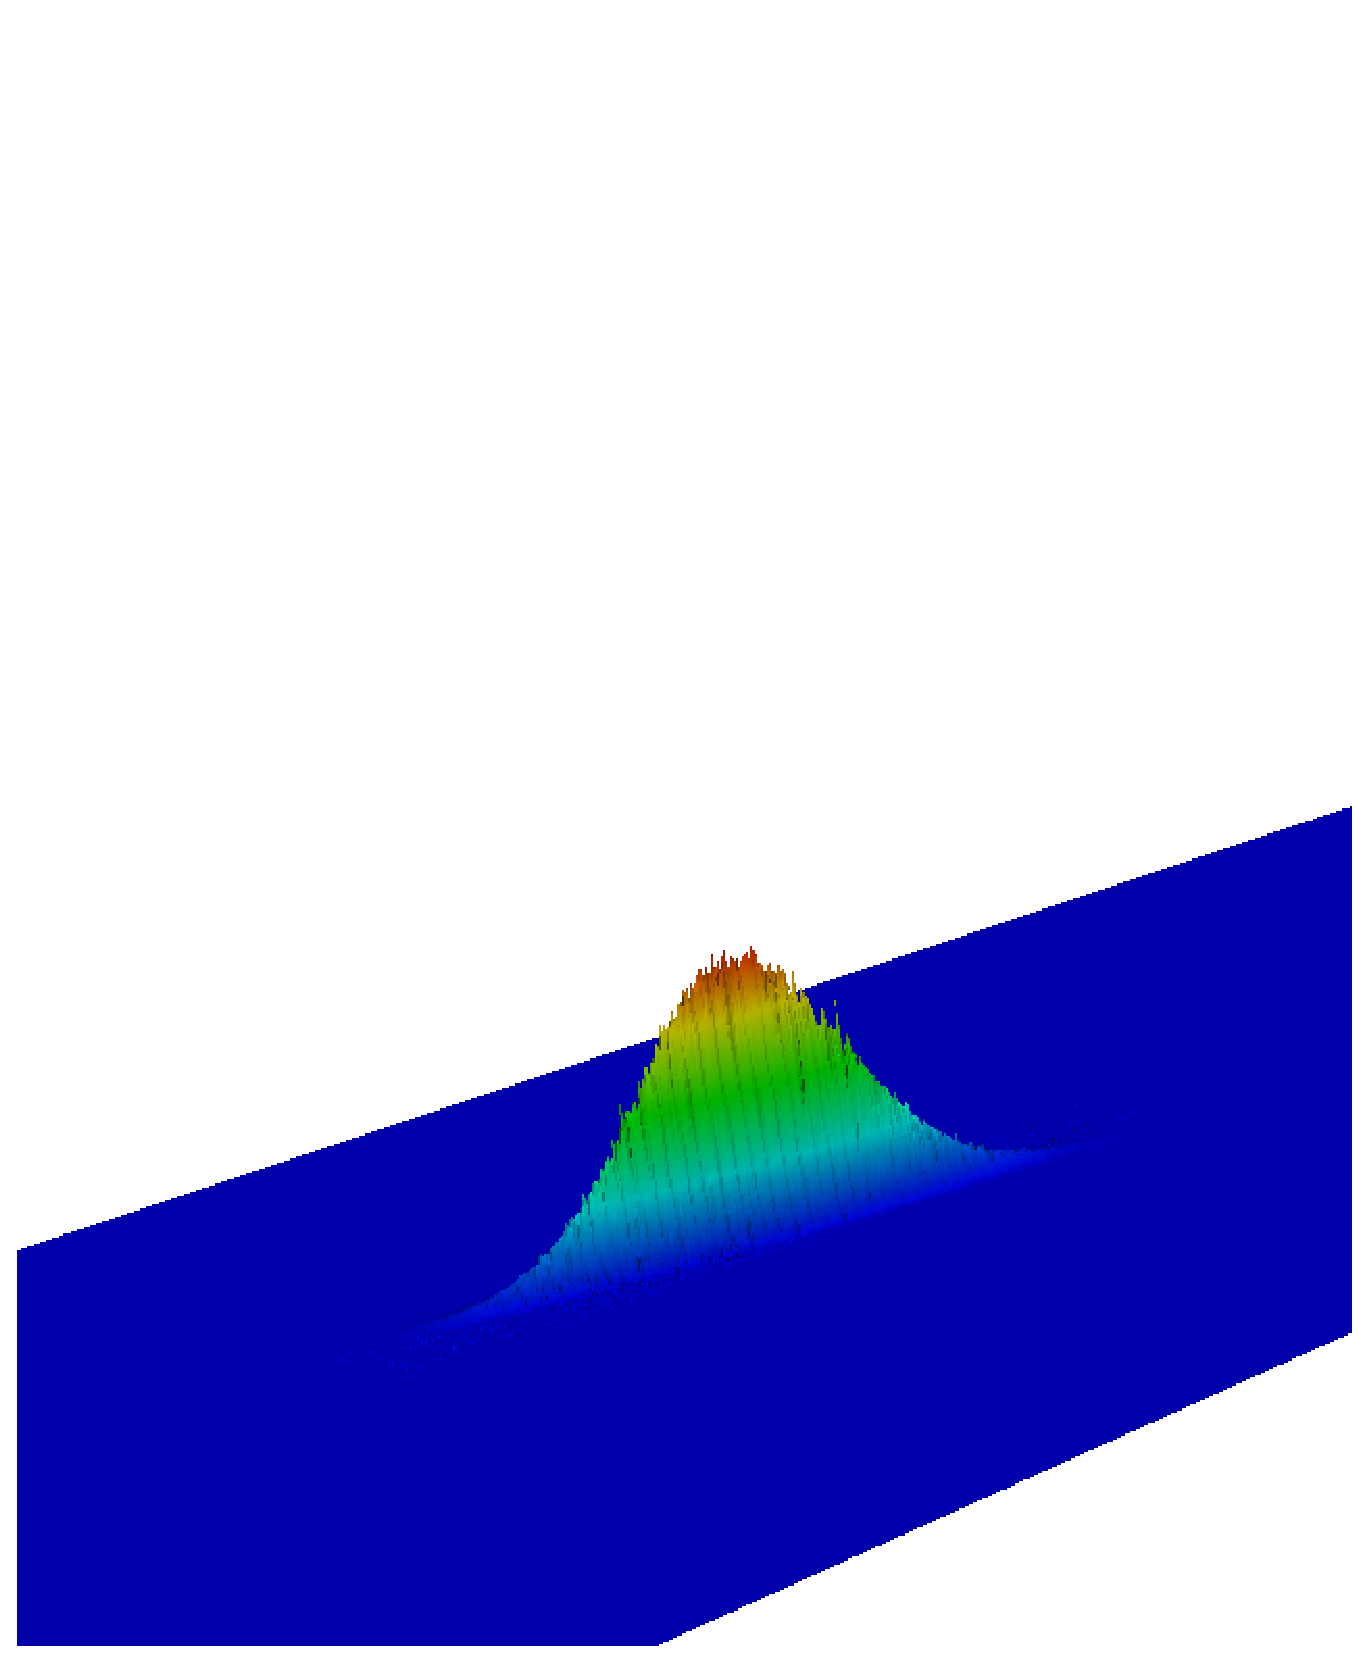
\includegraphics[width=0.5\columnwidth]{figures/wiens_prop1.eps}
  }
  \subfigure
  {
  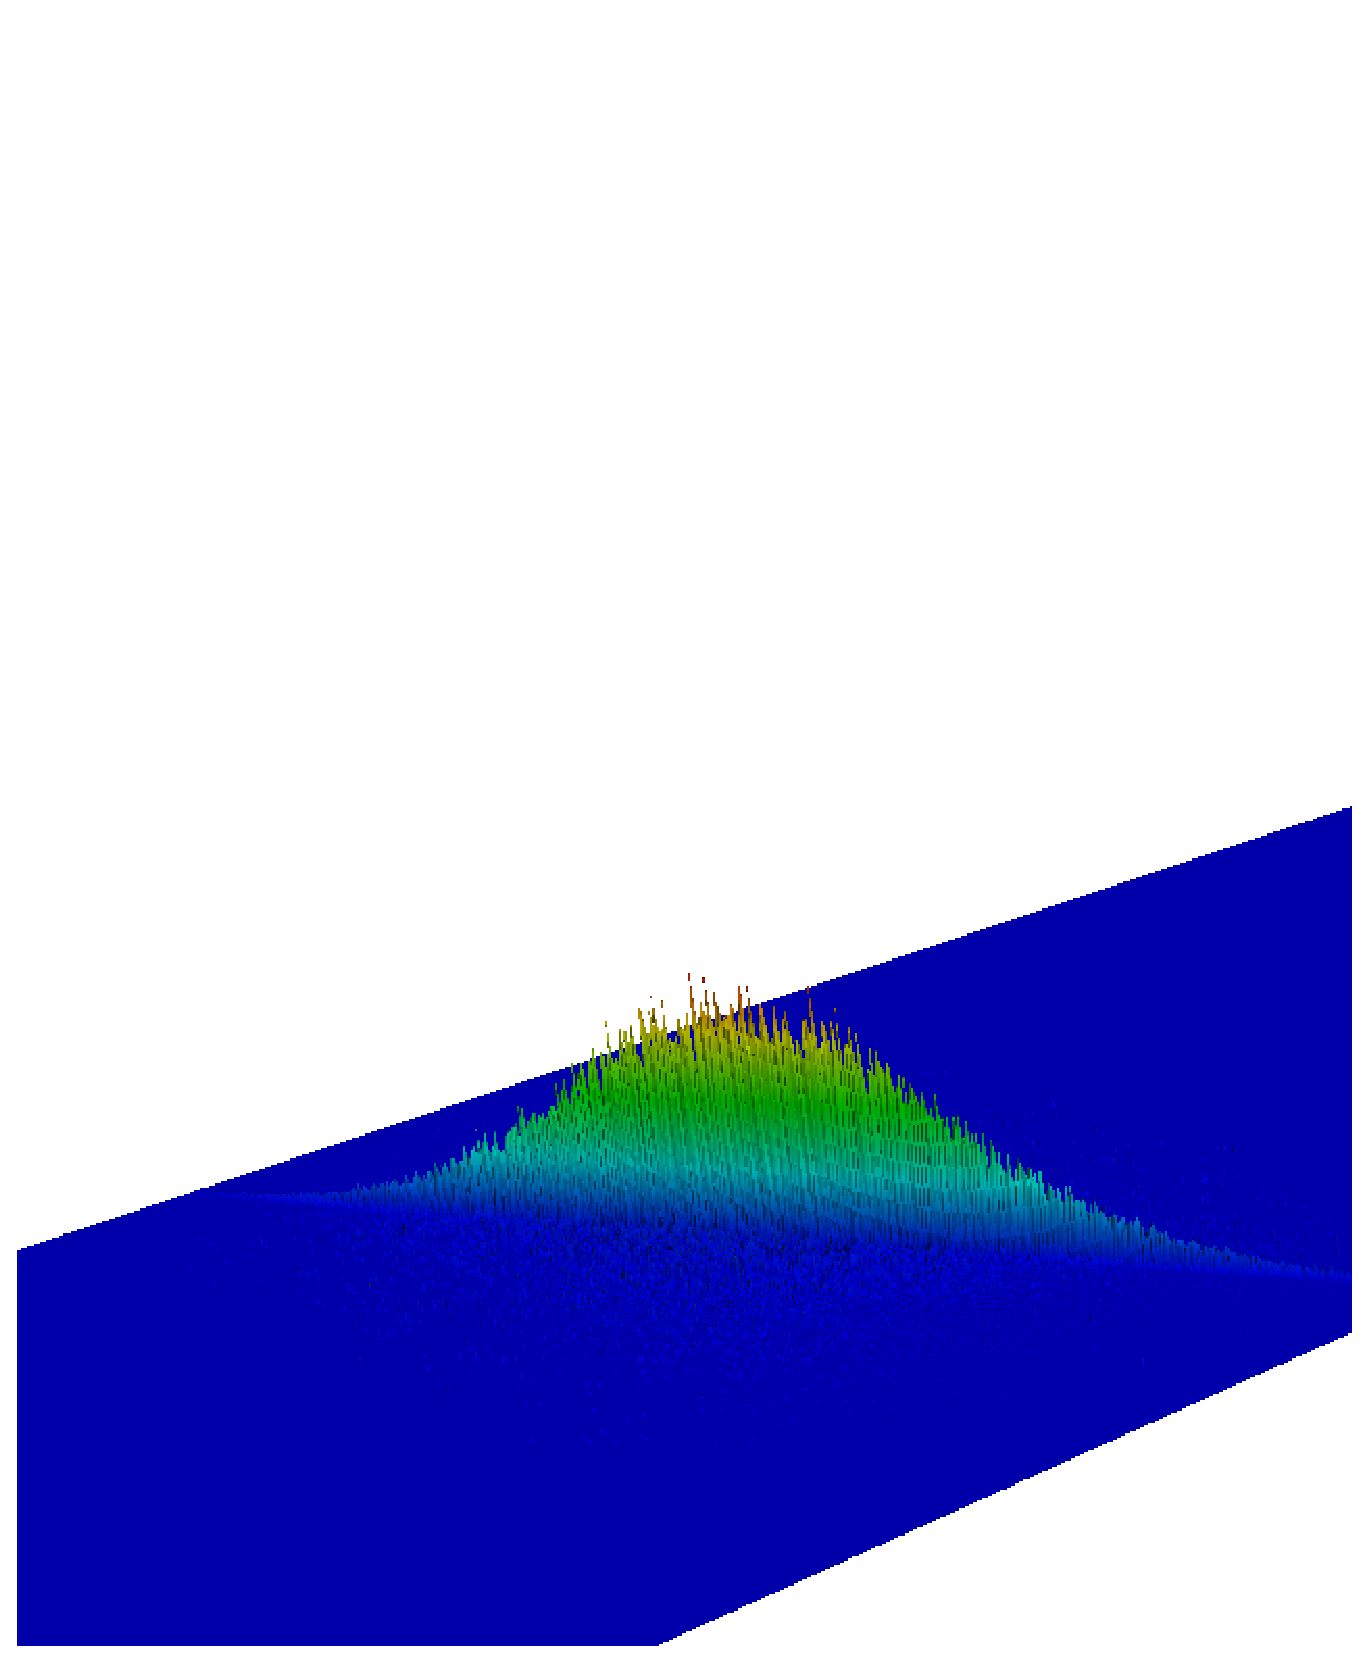
\includegraphics[width=0.5\columnwidth]{figures/wiens_prop9.eps}
  }
  \caption{
    Phase space distribution functions computed by the PD simulator are shown.
    In the classical case it can be interpreted directly
    as probability to find a particle, the indefinite nature in the
    quantum case, prohibits this direct interpretation, but still
    provides correct derived quantities such as density and momentum
    distribution. The evolution is shown at $100fs$ (\textbf{top})
    and at $1ps$ (\textbf{bottom}).
  }
  \label{fig:one}
\end{figure}

\clearpage

% ==============================================================================
% ==============================================================================
\section{Simulation Control} \label{wigner:sim}
% ==============================================================================
% ==============================================================================

The simulations are controlled via the input configuration and parameter XML files.
In the following the individual variables are explained in detail.

%\subsection{Parameters}



\begin{table}[ht!]
\centering
\begin{tabular}{|l|p{4.5cm}|c|c|}
\hline
\textbf{Variable}   & \textbf{Definition}   & \textbf{Unit} & \textbf{Default} \\
\hline
%\texttt{NI}  & FILLME & $m^{-3}$ & $1$ \\
%\hline
\texttt{TL}  & Lattice Temperature & $K$ & $300$ \\
\hline
%\texttt{Z}  &  FILLME  &  & $0.5e-12$ \\
%\hline
\texttt{effmass}  & Effective Mass Factor &  & $0.067$ \\
\hline
\texttt{alpha}  & Non-Parabolicity Factor & $1/eV$ & $0.61$ \\
\hline
\texttt{rho}  & Density & $kg/m^3$ &$5.36e3$ \\
\hline
%\texttt{us}  &  FILLME  & $m/s$ &$1./3. * ( 2. * 3.0e3  + 5.24e3 )$ \\
%\hline
%\texttt{DA}  &  FILLME  & $eV$ &$7.0$ \\
%\hline
%\texttt{energy\_beta}  &  FILLME  & $J$ &$1$ \\
%\hline
%\texttt{DO}  & FILLME   & $J/m$ &$1$ \\
%\hline
\texttt{optical\_phonon\_energy}  &  Optical Phonon Energy  & $eV$ &$0.0343$ \\
\hline
\texttt{polar\_optical\_phonon\_energy}  &  Polar Optical Phonon Energy  & $eV$ &$0.036$\\
\hline
\texttt{optical\_permitivity}  &  Optical Permitivity  & & $10.92$ \\
\hline
\texttt{static\_permitivity}  & Static Permitivity   & & $12.9$ \\
\hline
\texttt{free\_flight\_coeff}  &  Free Flight Coefficient  & $1/Hz$ & $1. / 2.6e13$ \\
\hline
\end{tabular}
\caption{The parameter variables are shown.}
\label{tab:paras}
\end{table}


%\subsection{Configuration}

%\clearpage

\begin{table}[ht!]
\centering
\begin{tabular}{|l|p{5cm}|c|c|}
\hline
\textbf{Variable}   & \textbf{Definition}   & \textbf{Unit} &\textbf{Default} \\
\hline
%\texttt{L}  &  FILLME   & m & 800 * 1e-9 \\
%\hline
%\texttt{p\_max}  &   FILLME  & 1/m & 6e-9 \\
%\hline
\texttt{x\_count}  & Number of simulation domain points in x-direction &  & 400 \\
\hline
\texttt{y\_count}  & Number of simulation domain points in y-direction &  & 3000 \\
\hline
\texttt{timestep}  & The time difference between two time steps &  s & 100.0e-15 \\
\hline
\texttt{max\_iterations}  & Number of simulated time steps &  & 10 \\
\hline
\texttt{max\_particle\_count}  &  Number of generated particles for each point in the phase space   &  & 30 \\
\hline
\end{tabular}
\caption{The configuration variables are shown.}
\label{tab:configs}
\end{table}

\clearpage

% ==============================================================================
\section{License}
% ==============================================================================

Boost Software License - Version 1.0 - August 17th, 2003

Permission is hereby granted, free of charge, to any person or organization
obtaining a copy of the software and accompanying documentation covered by
this license (the "Software") to use, reproduce, display, distribute,
execute, and transmit the Software, and to prepare derivative works of the
Software, and to permit third-parties to whom the Software is furnished to
do so, all subject to the following:

The copyright notices in the Software and this entire statement, including
the above license grant, this restriction and the following disclaimer,
must be included in all copies of the Software, in whole or in part, and
all derivative works of the Software, unless such copies or derivative
works are solely in the form of machine-executable object code generated by
a source language processor.

THE SOFTWARE IS PROVIDED "AS IS", WITHOUT WARRANTY OF ANY KIND, EXPRESS OR
IMPLIED, INCLUDING BUT NOT LIMITED TO THE WARRANTIES OF MERCHANTABILITY,
FITNESS FOR A PARTICULAR PURPOSE, TITLE AND NON-INFRINGEMENT. IN NO EVENT
SHALL THE COPYRIGHT HOLDERS OR ANYONE DISTRIBUTING THE SOFTWARE BE LIABLE
FOR ANY DAMAGES OR OTHER LIABILITY, WHETHER IN CONTRACT, TORT OR OTHERWISE,
ARISING FROM, OUT OF OR IN CONNECTION WITH THE SOFTWARE OR THE USE OR OTHER
DEALINGS IN THE SOFTWARE.
